\documentclass[a4paper]{article}
\usepackage[14pt]{extsizes} 
\usepackage[T2A]{fontenc}
\usepackage[utf8]{inputenc}
\usepackage{natbib}
\usepackage{graphicx}
\usepackage{amsmath}
\usepackage[english, russian]{babel}
\usepackage{amsmath,amsfonts,amssymb,amsthm,mathtools,mathrsfs}
\usepackage{icomma}
\usepackage{fullpage}
\usepackage{ulem}
\usepackage{eufrak}
\usepackage{setspace}
\usepackage{listings}
\usepackage{indentfirst}
\usepackage[left=2cm,right=1.5cm,top=2cm,bottom=2cm]{geometry}
\usepackage{xcolor}
\usepackage{float}
\usepackage{csquotes}

\setlength{\parindent}{5ex}
\setlength{\parskip}{1em}
\renewcommand{\baselinestretch}{1}

\graphicspath{{images/}}

\definecolor{buzzlightyear}{HTML}{8757A5}
\definecolor{grass}{HTML}{738D06}
\definecolor{literal}{HTML}{F18A2B}
\definecolor{commentcolor}{HTML}{8E908B}

\lstdefinestyle{habrstyle}{
    backgroundcolor=\color{white},   
    commentstyle=\color{commentcolor},
    keywordstyle=\bfseries\color{buzzlightyear},
    numberstyle=\tiny\color{commentcolor},
    stringstyle=\color{grass},
    basicstyle=\ttfamily\footnotesize,
    breakatwhitespace=false,         
    breaklines=true,                 
    captionpos=b,                    
    keepspaces=true,                 
    numbers=left,                    
    numbersep=5pt,                  
    showspaces=false,                
    showstringspaces=false,
    showtabs=false,                  
    tabsize=4
}

\lstset{style=habrstyle}

\begin{document}
    % НАЧАЛО ТИТУЛЬНОГО ЛИСТА
    \begin{center}
        \begin{center}
        \hfill \break
        \normalsize{Санкт-Петербургский государственный политехнический}\\
        \normalsize{университет Петра Великого}\\
        \hfill \break
        \normalsize{\textbf{Высшая школа интеллектуальных систем и}}\\ 
        \normalsize{\textbf{суперкомпьютерных технологий}}\\ 
        \hfill \break
        \hfill \break
        \hfill \break
        \normalsize{Лабораторная работа №11}\\
        \hfill \break
        \hfill \break
        \normalsize{\LARGE Модуляция и выборка (квантование)}\\
        \end{center}
        \hfill \break
        \hfill \break
        \hfill \break
        \hfill \break
        \hfill \break
        \hfill \break
        \hfill \break
        \hfill \break
        \hfill \break
        \hfill \break
        \begin{flushright}
            \normalsize{Выполнил студент 3-го курса}\\
            \normalsize{группа 3530901/80201}\\
            \normalsize{Матвеец Андрей Вадимович}\\
            \hfill \break
            \normalsize{Преподаватель:}\\
            \normalsize{Богач Наталья Владимировна}\\
        \end{flushright}
        \hfill \break
        \hfill \break
        \hfill \break
        \hfill \break
        \begin{center} Санкт-Петербург\end{center}
        \begin{center}2021\end{center} 
        \thispagestyle{empty}
    \end{center}
    % КОНЕЦ ТИТУЛЬНОГО ЛИСТА
    
    % ОГЛАВЛЕНИЕ
    \newpage
        \tableofcontents
    
    % СПИСОК ИЛЛЮСТРАЦИЙ
    \newpage
         \listoffigures
    
    % СПИСОК ЛИСТИНГОВ     
    \newpage
         \lstlistoflistings   
     
    \newpage
        \section{Часть №1: \texttt{chap11.ipynb}}
            В первой части лабораторной работы нам необходимо изучить и запустить весь код из блокнота \texttt{chap11.ipynb}.
            
            В результате выполнения данного пункта можно сказать, что все листинги из блокнота успешно запускаются:
            
            \begin{figure}[H]
                \centering
                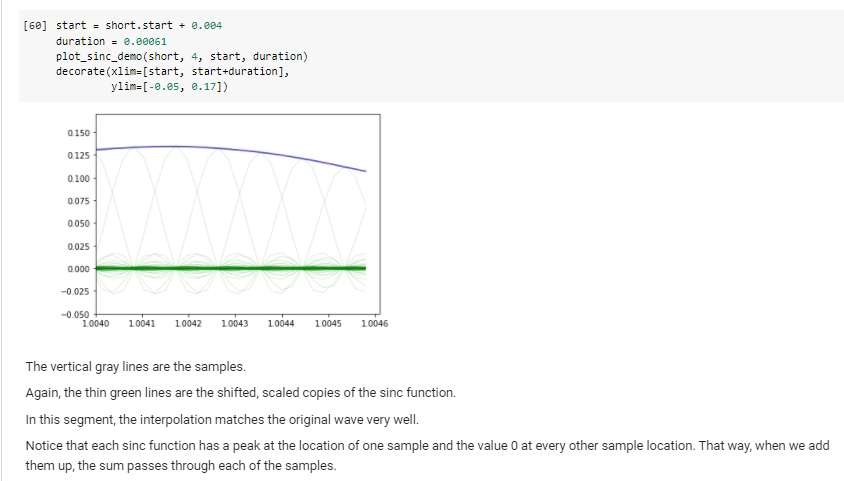
\includegraphics[width=\textwidth]{ex_1_1.png}
                \caption{Результат запуска блокнота \texttt{chap11.ipynb}}
                \label{fig:ex_1_1}
            \end{figure}
            
    \newpage
        \section{Часть №2: Крис "Монти" Монтгомери - "D/A and A/D | Digital Show and Tell"}
            Во втором пункте лабораторной работы нам необходимо просмотреть ролик Криса "Монти" Монтгомери - "D/A and A/D | Digital Show and Tell".
            
            В результате, после просмотра данного видеоролика мы выяснили, почему аналоговое аулио в приемлемых пределах человеческого слуха может воспроизводиться с идеальной точностью с использованием 16-битного цифрового сигнала 44.1 кГц.
            
    \newpage
        \section{Часть №3: "Соло на барабане" и фильтр НЧ}
            В третьем пункте  лабораторной работы нам необходимо применить фильтр НЧ к примеру "Соло на барабане" до выборки, после чего снова с помощью фильтра НЧ удалить спектральные копии, которые вызваны выборкой.
            
            Для начала получим нужный нам сигнал:
            
\begin{lstlisting}[language=Python, caption= Получение сигнала]
    wave = read_wave('263868__kevcio__amen-break-a-160-bpm.wav')
    wave.normalize()
    wave.plot()
\end{lstlisting}
            
            \begin{figure}[H]
                \centering
                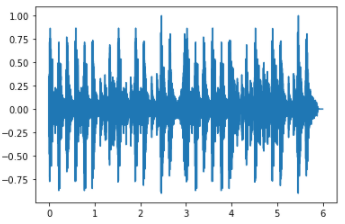
\includegraphics{ex_3_1.png}
                \caption{Полученный сигнал}
                \label{fig:ex_3_1}
            \end{figure}
            
            Сразу после этого переведем его в аудио:
            
            \begin{figure}[H]
                \centering
                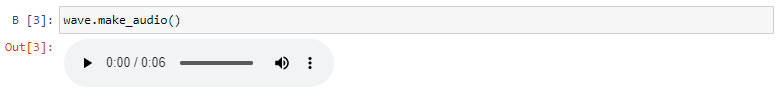
\includegraphics[width=\textwidth]{ex_3_2.png}
                \caption{Перевод полученного сигнала в аудио}
                \label{fig:ex_3_2}
            \end{figure}

            Теперь получим спектр данного сигнала:
            
\begin{lstlisting}[language=Python, caption= Получение спектра]
    spectrum = wave.make_spectrum(full=True)
    spectrum.plot()
\end{lstlisting}
            
            \begin{figure}[H]
                \centering
                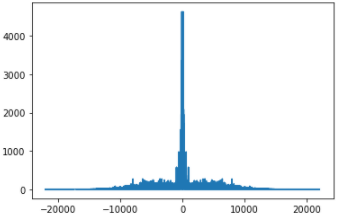
\includegraphics{ex_3_3.png}
                \caption{Полученный спектра}
                \label{fig:ex_3_3}
            \end{figure}
            
            Затем уменьшим частоту дискретизации в 3 раза:
            
\begin{lstlisting}[language=Python, caption= Уменьшение частоты дискретизации в 3 раза]
    factor = 3
    framerate = wave.framerate / factor
    cutoff = framerate / 2 - 1
\end{lstlisting}
            
            После этого нужно применить фильтр сглаживания для удаления частот выше новой частоты свертки:
            
\begin{lstlisting}[language=Python, caption= Применение фильтра]
    spectrum.low_pass(cutoff)
    spectrum.plot()
\end{lstlisting}
            
            \begin{figure}[H]
                \centering
                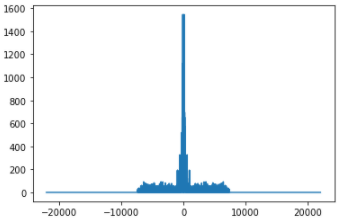
\includegraphics{ex_3_7.png}
                \caption{Применение фильтра}
                \label{fig:ex_3_7}
            \end{figure}
            
            \begin{figure}[H]
                \centering
                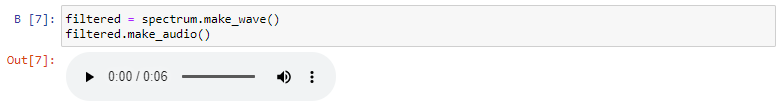
\includegraphics[width=\textwidth]{ex_3_4.png}
                \caption{Применение фильтра и результат}
                \label{fig:ex_3_4}
            \end{figure}
            
            Полученный сигнал все еще похож на исходный сигнал.
            
            Теперь напишем функцию \texttt{sample}, которая будет имитировать процесс выборки:
            
\begin{lstlisting}[language=Python, caption= Функция \texttt{sample}]
    def sample(wave, factor):
        ys = np.zeros(len(wave))
        ys[::factor] = np.real(wave.ys[::factor])
        return Wave(ys, framerate=wave.framerate)
\end{lstlisting}
            
            Сразу же проверим нашу функцию:
            
            \begin{figure}[H]
                \centering
                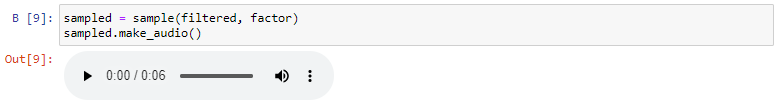
\includegraphics[width=\textwidth]{ex_3_5.png}
                \caption{Проверка функции \texttt{sample}}
                \label{fig:ex_3_5}
            \end{figure}
            
            Полученный сигнал полсе вызова функции должен содержать слабозаметные спектральные копии, которые можно увидеть, создав спектр данного сигнала:
            
\begin{lstlisting}[language=Python, caption= Создание спектра сигнала]
    sampled_spectrum = sampled.make_spectrum(full=True)
    sampled_spectrum.plot()
\end{lstlisting}
            
            \begin{figure}[H]
                \centering
                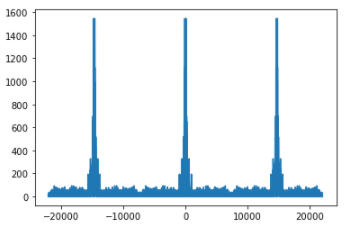
\includegraphics{ex_3_6.png}
                \caption{Полученный спектр}
                \label{fig:ex_3_6}
            \end{figure}
            
            На спектре можно увидеть спектральные копии. Чтобы их убрать нам необходимо применить фильтр сглаживания:
            
\begin{lstlisting}[language=Python, caption= Применение фильтра сглаживания]
    sampled_spectrum.low_pass(cutoff)
    sampled_spectrum.plot()
\end{lstlisting}
            
            \begin{figure}[H]
                \centering
                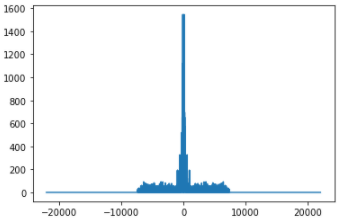
\includegraphics{ex_3_7.png}
                \caption{Примененный фильтр сглаживания}
                \label{fig:ex_3_7}
            \end{figure}
            
            Теперь масштабируем полученный спектр:
            
\begin{lstlisting}[language=Python, caption= Масштабирование спектра]
    sampled_spectrum.scale(factor)
    spectrum.plot()
    sampled_spectrum.plot()
\end{lstlisting}
            
            \begin{figure}[H]
                \centering
                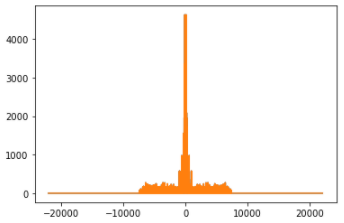
\includegraphics{ex_3_8.png}
                \caption{Масштабирование спектра}
                \label{fig:ex_3_8}
            \end{figure}
            
            После этого проверим разницу между спектром до и после фильтрации, после чего преобразуем спектр обратно в волну:
            
            \begin{figure}[H]
                \centering
                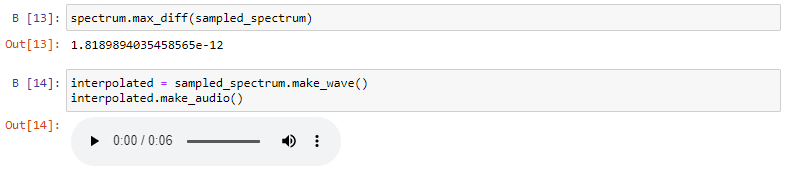
\includegraphics[width=\textwidth]{ex_3_9.png}
                \caption{Сравнение спектров и преобразование в волну}
                \label{fig:ex_3_9}
            \end{figure}
            
            И, наконец, посмотрим на полученный сигнал:
            
            \begin{figure}[H]
                \centering
                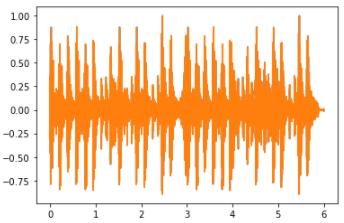
\includegraphics{ex_3_10.png}
                \caption{Результат}
                \label{fig:ex_3_10}
            \end{figure}
            
            По итогу можно сделать вывод о том, что разница между интерполированной и фильтрованной волной очень мала.
            
    \newpage
        \section{Выводы}
             В результате выполнения лабораторной работы мы разобрались со сверткой с импульсами, с выборкой и с фильтрацией спектров, изучили весь блокнот \texttt{chap11.ipynb}, также посмотрели видеоролик Криса "Монти" Монтгомери - "D/A and A/D | Digital Show and Tell", из которого мы узнали почему аналоговое аулио в приемлемых пределах человеческого слуха может воспроизводиться с идеальной точностью с использованием 16-битного цифрового сигнала 44.1 кГц. Также в последнем пункте мы на основе "Соло на барабане"  изменили фильтр НЧ до выборки и с помошью него же удалили спектральные копии, полученные в результате выборки.
             
\end{document}
